%\documentclass[12pt,a4paper]{report}
\documentclass[12pt,a4paper,oneside,onecolumn,openright]{book}
% set the document language
\usepackage[italian]{babel}
% set the encoding used by your editor here (default is utf8)
\usepackage[utf8]{inputenc}
\usepackage[T1]{fontenc}

% math packages
\usepackage{amsmath}
\usepackage{amssymb}
\usepackage{lmodern}
\usepackage{varwidth}
\usepackage{xcolor}
\usepackage[makeroom]{cancel}
% page margins settings
\usepackage[inner=1.5cm,outer=1.5cm,top=1.5cm,bottom=1.5cm]{geometry}
%\usepackage{indentfirst}

% other packages
\usepackage{array}
\usepackage{enumitem}
\usepackage{subfigure}
\usepackage{graphicx}
\usepackage{verbatim}
\usepackage{listings}
\usepackage{url}
\usepackage[hidelinks]{hyperref}
\usepackage[export]{adjustbox}
\usepackage{latexsym}
\usepackage{tabularx}
\usepackage{ragged2e}
\usepackage{mathtools}
\DeclarePairedDelimiter\floor{\lfloor}{\rfloor}
\DeclarePairedDelimiter\ceil{\lceil}{\rceil}
% \usepackage{Mathematics}
% custom colors
\usepackage{color}
\usepackage{wrapfig}
\usepackage{gensymb}
\usepackage{caption}
\usepackage{tikz}
\usepackage{forest}
\usepackage{tikz-qtree}

\newcommand\myeq{\stackrel{\mathclap{\tiny\mbox{def}}}{=}}

\usepackage[many]{tcolorbox}
\newtcolorbox{boxA}{
    % fontupper = \bf,
    boxrule = 1.5pt,
    colframe = black % frame color
}

\usetikzlibrary{shadows}
\definecolor{light-gray}{gray}{0.96}
\definecolor{cyan}{RGB}{230,230,255}
\definecolor{dkgreen}{rgb}{0,0.6,0}
\definecolor{gray}{rgb}{0.5,0.5,0.5}
\definecolor{mauve}{rgb}{0.58,0,0.82}
\definecolor{iceberg}{rgb}{0.44, 0.65, 0.82}
% \definecolor{blue}{RGB}{44, 44, 210}

\hypersetup{
colorlinks=true,
linkcolor=black,
% filecolor=blue,
urlcolor=blue,
% pdftitle={Overleaf Example},
}

\urlstyle{same}
\graphicspath{ {./images/} }

% environment for bash code
\lstset{ %
  language=bash,                % the language of the code
  basicstyle=\footnotesize,           % the size of the fonts that are used for the code
  numbers=left,                   % where to put the line-numbers
  numberstyle=\footnotesize,          % the size of the fonts that are used for the line-numbers
  stepnumber=1,                   % the step between two line-numbers. If it's 1, each line 
                                  % will be numbered
  numbersep=5pt,                  % how far the line-numbers are from the code
  backgroundcolor=\color{white},      % choose the background color. You must add \usepackage{color}
  showspaces=false,               % show spaces adding particular underscores
  showstringspaces=false,         % underline spaces within strings
  showtabs=false,                 % show tabs within strings adding particular underscores
%  frame=single,                   % adds a frame around the code
  rulecolor=\color{black},        % if not set, the frame-color may be changed on line-breaks within not-black text (e.g. commens (green here))
  tabsize=2,                      % sets default tabsize to 2 spaces
  captionpos=b,                   % sets the caption-position to bottom
  breaklines=true,                % sets automatic line breaking
  breakatwhitespace=false,        % sets if automatic breaks should only happen at whitespace
  title=\lstname,                   % show the filename of files included with \lstinputlisting;
                                  % also try caption instead of title
  numberstyle=\tiny\color{gray},        % line number style
  keywordstyle=\textbf,          % keyword style
  commentstyle=\color{dkgreen},       % comment style
%  stringstyle=\color{mauve},         % string literal style
  escapeinside={\%*}{*)},            % if you want to add a comment within your code
  morekeywords={*,...,insert,-}               % if you want to add more keywords to the setù
}

% environment for python code
\lstset{
	language=Python,
	breaklines=true,
	breakatwhitespace=true ,
	backgroundcolor=\color{light-gray}
}

\newcommand{\grayScale}{0.95} % Can change the gray level here
\definecolor{codeBackground}{rgb}{\grayScale ,\grayScale ,\grayScale}
\definecolor{forestGreen}{rgb}{0.13,0.55,0.13}

\lstset{
    language=C,
    backgroundcolor=\color{codeBackground},
    tabsize=4,
    showstringspaces=false,
    showtabs=false,
    showspaces=false,
    basicstyle=\ttfamily,
    identifierstyle=\ttfamily,
    keywordstyle=\color{blue},
    stringstyle=\color{red},
    commentstyle=\color{gray},
    numberstyle=\color{magenta},
    morecomment=[l][\color{forestGreen}]{\#},
    escapechar={|}, 
}
% appendices package
%\usepackage{appendix}
% set Appendix name used in the toc
%\renewcommand{\appendixtocname}{Appendice}

% interline
\linespread{1.5}
% set numbers for subsections and show them in the toc
\setcounter{tocdepth}{3} 
\setcounter{secnumdepth}{3}

% layout package, style and settings
\usepackage{fancyhdr}
\pagestyle{fancy}

\fancypagestyle{mainmatter}{%		
		\fancyhf{} 
		\fancyhead{}
		\fancyhead[LE,RO]{\thepage}
		\fancyhead[LO]{\footnotesize{\leftmark}}
		\fancyhead[RE]{\footnotesize{\rightmark}}
		\fancyfoot{}
		\addtolength{\headwidth}{\marginparsep}
		\addtolength{\headheight}{2.5pt}
		\renewcommand{\headrulewidth}{0.3pt}
		\renewcommand{\footrulewidth}{0.0pt}
		}
\fancypagestyle{frontmatter}{%
		\fancyhf{} 
		\fancyhead[LE]{\footnotesize{\MakeUppercase{\thepage}}}
		\fancyhead[RO]{\footnotesize{\MakeUppercase{\thepage}}}
		\fancyhead[RE,LO]{}
		\fancyfoot{}
		\addtolength{\headwidth}{\marginparsep}
		\addtolength{\headheight}{2.5pt}
		\renewcommand{\headrulewidth}{0.0pt}
		\renewcommand{\footrulewidth}{0.0pt}
		}
		
		
\usepackage{fancyhdr}
\pagestyle{fancy}
		\fancyhf{} 
		\fancyhead{}
		\fancyhead[LE,RO]{\thepage} 
		\fancyhead[LO]{\footnotesize{\leftmark}}
		\fancyhead[RE]{\footnotesize{\rightmark}}
		\fancyfoot{}
		\addtolength{\headwidth}{\marginparsep}
		\addtolength{\headheight}{2.5pt}
		\renewcommand{\headrulewidth}{0.3pt}
		\renewcommand{\footrulewidth}{0.0pt}

% empty pages have no numbers
\makeatletter
\def\cleardoublepage{\clearpage\if@twoside \ifodd\c@page\else
\hbox{}
  %Potresti voler togliere il commento dalla linea seguente
  %Questa pagina � stata lasciata intenzionalmente vuota.
\thispagestyle{empty}
\newpage
\if@twocolumn\hbox{}\newpage\fi\fi\fi}
\makeatother
%????
%\textwidth=450pt\oddsidemargin=0pt

%\makeatletter 
%  \DeclareRobustCommand*\textsubscript[1]{% 
%    \@textsubscript{\selectfont#1}} 
%  \newcommand{\@textsubscript}[1]{% 
%    {\m@th\ensuremath{_{\mbox{\fontsize\sf@size\z@#1}}}}} 
\makeatother 

\begin{document}
\begin{titlepage}
\begin{center}
{
    \large
    \textbf{Università  degli studi di Modena e Reggio Emilia} \\
   	\textbf{Dipartimento di Ingegneria Enzo Ferrari} \\
    \vspace{\stretch{0.5}}
    \hspace*{0cm} \hrulefill \hspace*{0cm} \\
    \vspace{\stretch{0.5}}    
	  \vspace{\stretch{12}}
  
  
 		\huge{\bf Matematica Discreta }}\\
		\vspace{3mm}
		
		\vspace{\stretch{6}}
		\end{center}
		
\vspace{40mm}
\par
\noindent
\vspace{20mm}
\begin{center}
\hspace*{0cm} \hrulefill \hspace*{0cm} \\
{\large{\bf 
Anno Accademico 2023/24}}
\end{center}

\end{titlepage}

\pagestyle{frontmatter}
\frontmatter

% PAGINA VUOTA
%\clearpage\null\thispagestyle{empty}\clearpage
\setcounter{tocdepth}{2}
\tableofcontents

\setlength{\parindent}{12pt}
\setlength{\parskip}{1ex plus 0.5ex minus 0.2ex}
\mainmatter
\pagestyle{mainmatter}

\chapter{Introduction}

\section{Structure and Content}
\begin{itemize}

    \item \textbf{Module 1}: 
    \begin{enumerate}
        \item \textbf{\textit{intra-vehicles communications}}: nodes, sensors, ECU
        \item \textbf{\textit{signal busses}}: CAN, LIN, FlexRay, MOST, Ethernet [ T1/T1S]
        \item \textbf{\textit{car domain and OS}}
    \end{enumerate}
    
    \item \textbf{Module 2}:
    \begin{enumerate}
        \item \textbf{\textit{inter-vehicles communications}}: \textit{V2V} and \textit{V2X} (car is a node)
        \item \textbf{\textit{wireless technologies}}: Bluetooth, LoRa, C-V2X, IEE 802.11p (bd)
        \item application, messages, broadcast, GPS
    \end{enumerate}

\end{itemize}
Different \textbf{domain} or \textbf{application} needs different \textit{communications protocols}, is important to understand how each nodes in domain communicate each other (inside the car).

\newpage
\section{Intra-Vehicles}
From the 80's, where the car's control unit are isolated an there was a dedicated wires connect sensors and actuators with less electronic than now, until the reach the greates goal of evolution in the automotive sector: autonomous drive. The complexity of the number of connection from each ECU's to the other, also the number of ECU's for each car, is growing. While the number of signal increase in a liner way, the connection between ECU's is growing with a quadratic complexity $O(n^2)$.

If we examine the evolutions of the ECUs number inside an ``Audi A6'' we can observe that in 1997 it has 5 ECUs and in the 2007 it has 50 ECUs, instead the ``Tesla M3'' in the 2017 has 70 ECUs. The quadratic increase of ECUs number, however has reach a cap for two main reason: the cost and the space inside the car. Traditionally one ECUs is responsible of one task, but nowadays it could be two type of trends:
\begin{enumerate}[nosep]
    \item \textit{distributed of function across ECUs}
    \item \textit{integration of multiple function in one ECU}
\end{enumerate}

\section{Architectures}

\begin{figure}[h]
    \centering
    \begin{minipage}[t]{0.45\textwidth}
        \centering
        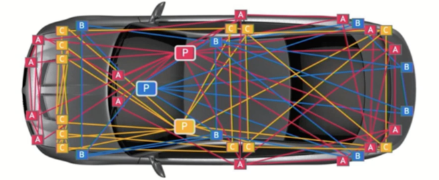
\includegraphics[width=\textwidth]{img/domain_architecture}
        \caption{\textit{Domain Architecture}}
        
        \begin{flushleft}
            \begin{enumerate}[nosep]
                \item central domain controller (\textbf{P}) or high performance computer
                \item ability to handle more complex functions
                \item cost optimization
                \item cable harness is rigid and expensive
            \end{enumerate}
        \end{flushleft}

    \end{minipage}
    \begin{minipage}[t]{0.45\textwidth}
        \centering
        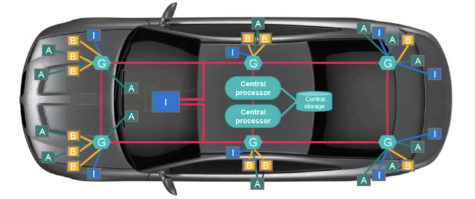
\includegraphics[width=\textwidth]{img/zonal_architecture}
        \caption{\textit{Zonal Architecture}}
        
        \begin{flushleft}
            \begin{enumerate}[nosep]
                \item local ethernet per zone (\textbf{G})
                \item ultra high-speed secured backbone between zone
                \item centralized software
                \item central computer storage
            \end{enumerate}
        \end{flushleft}
        
    \end{minipage}
\end{figure}
\chapter{Parte 3}
\section{Strutture algebriche elementari}
Una \textbf{operazione binaria intera} su un insieme G è un'applicazione 
\begin{center}
    $\ast \; : \; G \times G \rightarrow G$
\end{center}
L'immagine della coppia $(x,y)$ si denoterà con $x \ast y$. 
\begin{itemize}
    \item $e \in G$ si dice \textbf{elemento neutro} rispetto a $\ast$ se:
    \begin{center}
        $g \ast e = e \ast g = g \; \forall g \in G$
    \end{center}
    \item un elemento $g \in G$ si dice invertibile se esiste $\bar{g} \in G$ tale che $g * \bar{g} = \bar{g} * g = e$
\end{itemize}

\subsection{Gruppi}
La coppia $(G, \ast)$, con $\ast$ operazione su G, si dice \textbf{gruppo} se vengono rispettate le seguenti proprietà:
\begin{itemize}
    \item $\ast$ è \textbf{associativa}: $\forall g, g', g'' \in G$ si ha $(g \ast g') \ast g'' = g \ast (g' \ast g'')$
    \item esiste l'elemento \textbf{neutro}
    \item ogni elemento di G è invertibile
\end{itemize}
Il gruppo si dice \textbf{abeliano} o \textbf{commutativo} se: 
\begin{center}
    $\forall g, g' \in G, \; g \ast g' = g' \ast g$ (proprietà \textbf{commutativa})
\end{center}
Alcuni \textcolor{yellow}{\textbf{esempi}}:
\begin{itemize}
    \item $(\mathbb{N}, +)$, $(\mathbb{Z}, \cdot)$ non sono gruppi. in quanto non né in $\mathbb{N}$ e $\mathbb{Z}$ sono presenti per ogni elemento dell'insieme dell'elemento inverso, in $\mathbb{N}$ non sono presenti elementi negativi, quindi nessun elemento avrà un'altro che sommato a se stesso dia 0, viceversa l'insieme $\mathbb{Z}$ che sono presenti elementi positivi e negativi viene definita l'operazione $\cdot$ richiede i reciproci dei singoli elementi affiché possano essere definiti gli elementi inversi.
    \item $(\mathbb{Z}, +)$, $(\mathbb{Q}, \cdot)$ sono gruppi abelliani
\end{itemize}

\subsection{Anelli}
La terna $(\mathbb{A}, +, \cdot)$ con $\mathbb{A}$ un insieme e $+, \cdot$ (somma e prodotto) due operazione binarie interne a $\mathbb{A}$, si dice \textbf{anello} se:
\begin{itemize}
    \item $(\mathbb{A}, +, \cdot)$ è un gruppo \textbf{abeliano} (con elemento neutro 0).
    \item il prodotto è \textbf{associativo}.
    \item per ogni $x,y,z \in \mathbb{K}$ si ha $x \cdot (y + z) = (x \cdot y) + (x \cdot z)$ e $(x + y) \cdot z = (x \cdot z) + (y \cdot z)$ (il prodotto è distribuito rispetto alla somma).
\end{itemize}
Un anello $(\mathbb{A}, +, \cdot)$ è detto \textbf{commutativa} se il prodotto è commutativo, mentre è detto \textbf{unitario} o con \textbf{unità} se $(\mathbb{A}, \cdot)$ ammette l'elemento neutro. $(\mathbb{Z}, +, \cdot)$, $(\mathbb{Q}, +, \cdot)$, $(\mathbb{R}, +, \cdot)$, $(\mathbb{C}, +, \cdot)$ sono anelli.

\newpage
\subsection{Campi}
La terna $(\mathbb{K}, +, \cdot)$ con $\mathbb{K}$ un insieme e $+, \cdot$ (somma e prodotto) due operazioni binarie interne a $\mathbb{K}$, si dice \textbf{campo} se:
\begin{itemize}
    \item $(\mathbb{K}, +)$ è un gruppo \textbf{abeliano} (con elemento neutro 0).
    \item $(\mathbb{K} - \{0\}, \cdot)$ è un gruppo \textbf{abeliano} (con elemento neutro 1).
    \item per ogni $x,y,z \in \mathbb{K}$ si ha $x \cdot (y + z) = (x \cdot y) + (x \cdot z)$ quindi il prodotto è distribuito rispetto alla somma.
\end{itemize}
In qualunque campo vale la \textbf{legge di annullamento del prodotto}:
\begin{center}
    $x \cdot y = 0 \rightarrow x = 0 \; \text{oppure} \; y = 0$
\end{center}

\subsection{Domini d'integrità}
\textbf{Divisori dello zero}: sia $(A, +, \cdot)$ un anello. Due elementi $a,b \in A$ si dicono \textbf{divisori dello zero} se $a \neq 0$, $b \neq 0$, ma $a \cdot b = 0$. Ad \textcolor{yellow}{\textbf{esempio}} l'anello delle matrici quadrate presenta dei divisori dello zero. \\
Un anello commutativo privo di divisori dello zero si dice \textbf{dominio di integrità}, ad \textcolor{yellow}{\textbf{esempio}} $(\mathbb{Z}, +, \cdot)$ è un anello commutativo unitario privo di divisori dello zero. Quindi è dominio di integrità.

\section{L'anello dei numeri interi}
È noto che $\exists h \; | \; h : \mathbb{Z} \rightarrow \frac{\mathbb{N}_0 \times \mathbb{N}_0}{\mathcal{R}}$ dove la relazione di equivalenza che si vuole definire è $\equiv_n$. Su questo insieme vengono \textbf{ben poste} le seguenti operazioni:
\begin{center}
    $\boxplus : \mathbb{Z} \times \mathbb{Z} \rightarrow \mathbb{Z}$ \\
    $((m, n), (m', n')) \mapsto [(m, n)] \boxplus [(m', n')] \myeq [(m + m', n + n')]$

    $\boxdot : \mathbb{Z} \times \mathbb{Z} \rightarrow \mathbb{Z}$ \\
    $((m, n), (m', n')) \mapsto [(m, n)] \boxdot [(m', n')] \myeq [(mm' + nn', mn' + m'n)]$
\end{center}
Definito questo possiamo dire che $(\mathbb{Z}, \boxplus, \boxdot)$ è \textbf{dominio di integrità}.

\section{Teoria della Divisibilità}
\textbf{Divisibilità}: dati due numeri $a,b \in \mathbb{Z}$, si dice che $a$ \textbf{divide} $b$ (e si scrive $a|b$) se:
\begin{center}
    $\exists c \in \mathbb{Z} \; | \; b = a \cdot c$
\end{center}
\textbf{Transitività}: se $n|m$ e $m|q$ allora $n|q$. \\
\textcolor{green}{\textbf{Dimostrazione}}: per ipotesi $\exists h \in \mathbb{Z} \; | \; m = h \cdot n$ e $\exists h' \in \mathbb{Z} \; | \; q = h' \cdot m$. Sostituendo la prima relazione nella seconda si ottiene $q = h' \cdot h \cdot n$. Poichè $h' \cdot h \in \mathbb{Z}$ abbiamo definito che $n|q$. \\ \newline
Se $n|m$ e $m|n$, allora $m \pm n$. \\
\textcolor{green}{\textbf{Dimostrazione}}: per ipotesi $\exists h \in \mathbb{Z} \; | \; m = h \cdot n$ e $\exists h' \in \mathbb{Z} \; | \; n = h' \cdot m$ andiamo a sostituire la seconda alla prima equazione:
\begin{center}
    \begin{align*}
        n &= h' \cdot h \cdot m \\
        n - h' \cdot h \cdot m &= 0 \\
        n \cdot (1 - h' \cdot h) &= 0
    \end{align*}
\end{center}
Essendo che $\mathbb{Z}$ è un \textbf{dominio di integrità}, segue che o $n = 0$ oppure $(1 - h' \cdot h) = 0 \rightarrow (h' \cdot h) = 1$, consideriamo che $n \leq 0$ e che quindi $h' \cdot h = 1$ sappiamo che $h$ ammette un inverso $h'$, da cui $h = h' = 1$ o $h = h' = -1$ (in $\mathbb{Z}$, gli unici elementi che ammettono inverso sono $1$ e $-1$). In questo modo sappiamo che $m=n$ oppure $m=-n$.

\section{Massimo Comune Divisore}
Dati $a,b \in \mathbb{Z}$ non entrambi nulli, si dice che $d \in \mathbb{Z}$ è \textbf{UN massimo comune divisore} tra $a$ e $b$ se:
\begin{itemize}
    \item $d|a$ e $d|b$
    \item $\forall d' \in \mathbb{Z} \; | \; d'|a, \; d'|b \Rightarrow d'|d$
\end{itemize}
Se $d$ e $d'$ sono due massimi comuni divisori tra $a$ e $b$ allora $d' = \pm d$.
\chapter{Aritmetica Modulare}
È nota la definizione di \textbf{insieme delle classi resto modulo $n$} $\mathbb{Z}_n \; (\forall n \in \mathbb{N}, n \geq 2)$, come insime quoziente di $\mathbb{Z}$ rispetto alla \textbf{relazione di congruenza} modulo $n$:

{\centering
    $a \equiv_n b \Longleftrightarrow \exists h \in \mathbb{Z} \; \text{t.c.} \; b - a = h \cdot n$
\par}
Inoltre:

{\centering
    $\mathbb{Z}_n = \frac{\mathbb{Z}}{\equiv_n} = \{[0], [1], ..., [n-1]\}$
\par}

\section{Operazioni in $\mathbb{Z}_n$}
Su $\mathbb{Z}_n = \frac{\mathbb{Z}}{\equiv_n}$ sono ben poste la \textbf{somma} e il \textbf{prodotto}

\subsection{Somma in $\mathbb{Z}_n$}

{\centering
    $\boxplus : \mathbb{Z}_n \times \mathbb{Z}_n \mapsto \mathbb{Z}_n$ \\
    $([a], [b]) \mapsto [a] \boxplus [b] \overset{\text{def}}{=} [a + b]$
\par}

\begin{boxA}
    \textcolor{olive}{\textbf{Dimostrazione}}: per provare che la somma è ben posta, occorre provare che, $\forall a' \in [a]$ e $\forall b' \in [b]$, si ha $[a' + b'] = [a + b]$. \\ 
    Per \textbf{Hp.} avremo che $\exists h \in \mathbb{Z} \; \text{t.c.} \; a' - a = h \cdot n$ ed $\exists h' \in \mathbb{Z} \; \text{t.c.} \; b' - b = h' \cdot n$. Facendo la somma otteniamo:

    {\centering
        $(a' - a) + (b' - b) = (h' \cdot n) + (h \cdot n)$ \\
        $(a' + b') - (a + b) = n \cdot \underset{\in \mathbb{Z}}{\fcolorbox{red}{white}{$(h' - h)$}}$
    \par}
    In questo modo siamo riusciti a provare la nostra \textbf{Th.}
\end{boxA}

\subsection{Prodotto in $\mathbb{Z}_n$}

{\centering
    $\boxdot : \mathbb{Z}_n \times \mathbb{Z}_n \mapsto \mathbb{Z}_n$ \\
    $([a], [b]) \mapsto [a] \boxdot [b] \overset{\text{def}}{=} [a \cdot b]$
\par}

\begin{boxA}
    \textcolor{olive}{\textbf{Dimostrazione}}: per provare che il prodotto è ben posto, occorre provare che $\forall a' \in [a]$ e $\forall b' \in [b]$, si ha $[a' \cdot b'] = [a \cdot b]$. \\
    Per \textbf{Hp.} avremo che $\exists h \in \mathbb{Z} \; \text{t.c.} \; a' - a = h \cdot n$ ed $\exists h' \in \mathbb{Z} \; \text{t.c.} \; b' - b = h' \cdot n$. Moltiplicando membro a membro $a' = a + hn$ e $b' = b + h'n$ otteniamo:

    {\centering
        $a' \cdot b' = (a + hn) \cdot (b + h'n) = ab + ah'n + bhn + hh'n^2$ \\
        $a'b' - ab = ah'n + bhn + hh'n^2 = n \cdot (\underset{\in \mathbb{Z}}{\fcolorbox{red}{white}{$ah' + bh + hh'n$}})$
    \par}
    In questo modo siamo riusciti a provare la nostra \textbf{Th.}
\end{boxA}

\begin{flushleft}
    \textbf{Proposizione}: $(\mathbb{Z}_n, \boxplus, \boxdot)$ è un anello commutativo con unità, $\forall n \in \mathbb{N}, n \geq 2$ 

    \textbf{Teorema}: $(\mathbb{Z}_n, \boxplus, \boxdot)$ è un campo \textit{se e solo se} $n$ è \textbf{primo}.

    \begin{boxA}
        \textcolor{olive}{\textbf{Dimostrazione}}
        
        \textcolor{red}{\textbf{Prima Parte}} ``$\Rightarrow$'': se $n$ non è primo avremo che $n = a \cdot b, \; \text{con} \; \{a, b\} \neq \{n, 1\}$ ma allora in $\mathbb{Z}_n$ avremo che $[a] \cdot [b] = [a \cdot b] = n = [0]$ il che significa che $\mathbb{Z}_n$ ammette divisori dello zero e quindi non può essere un campo.

        \textcolor{red}{\textbf{Seconda Parte}} ``$\Leftarrow$'': se $n$ è primo, bisogna dimostrare che ogni elemento non nullo ammette l'inverso. Si può dire che $[a] \neq [0] \Rightarrow a \not \equiv_n 0$ quindi che $a$ non è multiplo di $n$.

        Quindi il $\gcd (a, n) = 1$, quindi per l'\textbf{identità di bezout} $\exists \alpha, \beta \in \mathbb{Z} \; \text{t.c.} \; 1 = \alpha \cdot a + \beta \cdot n$ che si può riscrivere come:

        {\centering
            $1 - \underset{\in [1]}{\fcolorbox{red}{white}{$a \cdot \alpha$}} = n \cdot \beta$
        \par}
        Ma se $a \cdot \alpha \in [1]$ questo implica che $[a \cdot \alpha] = [1]$ ovvero $[a] \cdot [\alpha] = [1]$ e quindi siccome 1 è l'elemento neutro per la moltiplicazione, avremo che $[\alpha]$ è l'inverso.
    \end{boxA}

    Se $n$ non è primo, occorre prestare attenzione ai calcoli in $\mathbb{Z}_n$. Ad esempio:

    {\centering
        $3 \cdot 5 \equiv_9 3 \cdot 8$, ma non è vero che $5 \equiv_9 8$
    \par}
    \textbf{Teorema}: $a \cdot c \equiv b \cdot b$ (mod $n$) $\Rightarrow \; a \equiv b$ (mod $\frac{n}{d}$) con $d = \gcd (c, n)$ \\
    \textbf{Corollario}: se $\gcd (c, n) = 1 \; \Rightarrow \; a \equiv b$ (mod $n$). Nel caso di $n$ \textbf{primo} avremo che 
    
    {\centering
        $\forall c \in \mathbb{Z}_n, \; c \neq 0 \rightarrow \gcd (c, n) = 1$
    \par}
\end{flushleft}

\newpage
\begin{flushleft}
    \textbf{Teorema}: ogni numero intero $n$ è congruo modulo 9 alla somma delle sue cifre.
    
    \begin{boxA}
        \textcolor{olive}{\textbf{Dimostrazione}}: esplicitando la natura posizionale del sistema decimale avremo:
        \begin{align*}
            n &= a_0 + a_1 \cdot 10 + a_2 \cdot 10^2 + a_3 \cdot 10^3 + ... + a_k \cdot 10^k = \\
            &= a_0 + a_1 \cdot (1 + 9) + a_2 \cdot (1 + 99) + a_3 \cdot (1 + 999) + ...+ a_k \cdot (1 + \underset{k}{\underbrace{99...999}}) = \\
            &= (a_0 + a_1 + a_2 + a_3 + ... + a_k) + 9 \cdot a_1 + 99 \cdot a_2 + 999 \cdot a_3 + ... + \underset{k}{\underbrace{99...999}} = \\
            &= (a_0 + a_1 + a_2 + a_3 + ... + a_k) + 9 \cdot (a_1 + 11 a_2 + 111 a_3 + ... + \underset{k}{\underbrace{11...111} a_k})
        \end{align*}
        Quindi $n$ si ottiene dalla somma delle sue cifre, agiungendone un multiplo di 9 il che prova la tesi. \textbf{Conseguenza}: prova del nove.
    \end{boxA}

        \textbf{Proprietà}:
        \begin{itemize}[nosep]
            \item \textbf{Criterio di Divisibilità per 3} (\textit{per 9}): un numero intero è divisibile per 3 (\textit{per 9}) se e solo se la somma delle sue cifre è divisibile per 3 (\textit{per 9}).
            \begin{boxA}
                \textcolor{olive}{\textbf{Dimostrazione}} \\
                $n \equiv a_k + a_{k-1} + ... + a_0$ sia modulo 3 che modulo 9
            \end{boxA}
            
            \item \textbf{Criterio di Divisibilità per 2 e per 5}: un numero intero è divisibile per 2 (\textit{o per 5}) se e solo se la cifra delle unità $a_0$ è divisibile per 2 (\textit{o per 5}).
            \begin{boxA}
                \textcolor{olive}{\textbf{Dimostrazione}} \\
                Per ogni $k > 1, \; 10^k \equiv 10$ sia modulo 2 che modulo 5. Quindi di avrebbe $n \equiv a_0$ sia modulo 2 che modulo 5
            \end{boxA}
            
            \item \textbf{Criterio di Divisibilità per 4 e per 25}: un numero intero è divisibile per 4 (o per 25) se e solo se il numero $a_1a_0$ formato dalle sue ultime due cifre è divisibile per 4 (o per 25).
            \begin{boxA}
                \textcolor{olive}{\textbf{Dimostrazione}} \\
                $100 = 2^25^2 \equiv 0$ sia modulo 4 che modulo 25. Allora ogni intero $n$ è congruo modulo 4 o 25 se le ultime due cifre sono divisibili per 4 o per 25
            \end{boxA}

            \item \textbf{Criterio di Divisibilità per $2^r$}: un numero intero è divisibile per $2^r$ se e solo se $2^r$ divide il numero costituito dalle ultime $r$ cifre di $n$
            \begin{boxA}
                \textcolor{olive}{\textbf{Dimostrazione}} \\
                È sufficente osservare che $10^k = 2^k5^k \equiv 0$ (mod $2^r$) $\forall k \geq r$
            \end{boxA}

            \item \textbf{Criterio di Divisibilità per 11}: un numero intero è divisibile per 11 se e solo se è divisibile per 11 la somma a segni alterni delle sue cifre:
            
            {\centering
                $a_0 - a_1 + a_2 - ... + (-1)^k a_k \equiv 0$ mod 11
            \par}
            \begin{boxA}
                \textcolor{olive}{\textbf{Dimostrazione}}: basta osservare che:

                {\centering
                    $10 \equiv -1 \; \text{mod} \; 11$  $\Rightarrow$   
                    $\begin{cases}
                        10^{2p} \equiv 1 \; \text{mod} \; 11 \\
                        10^{2p + 1} \equiv -1 \; \text{mod} \; 11
                    \end{cases}$
                \par}
            \end{boxA}
            
        \end{itemize}
\end{flushleft}

\section{Congruenze Lineari}

\begin{flushleft}
    Si chiama \textbf{congruenza lineare} un'equazione di primo grado in $\mathbb{Z}_n$ a coefficienti interi:

    {\centering
        $a \cdot x \equiv b \; \text{mod} \; n \qquad \text{con} \; a, b, n \in \mathbb{Z}, n \geq 2$
    \par}
    Che equivale a $[a] \cdot [x] = [b]$ \\
    \textbf{Teorema dell'Esistenza di Soluzioni}: una congruenza lineare ammette soluzioni se e solo se $\gcd (a, n)|b$
    \begin{boxA}
        \textcolor{olive}{\textbf{Dimostrazione}}: ad ogni \textbf{congruenza lineare} è possibile associare un'\textbf{equazione diofantea}. Infatti:

        {\centering
            $ax \equiv b \; \text{mod} \; n \; \Longleftrightarrow \; \exists h \in \mathbb{Z} \; \text{t.c.} \; b - ax = hn$ ovvero \fcolorbox{red}{white}{$ax + hn = b$}
        \par}
        Quindi come condizione necessaria e sufficiente per la risolubilità della congruenza lineare è verificare la risolubilità dell'equazione diofantea associata è $\gcd (a, n)|b$ 
    \end{boxA}

    \textbf{Teorema per la Risoluzione di Congruenze Lineari}: sia $ax \equiv b \; \text{mod} \; n$ una congruenza lineare tale che $d|b$ con $d = \gcd (a, n)$ e sia \fcolorbox{red}{white}{$x_0$} una sua particolare risoluzione. Allora:
    \begin{itemize}[nosep]
        \item in $\mathbb{Z}$ le soluzioni sono tutti e soli gli interi del tipo:

        {\centering
            $x_0 + h \cdot \frac{n}{d}, \; h \in \mathbb{Z}$
        \par}
        \item in $\mathbb{Z}_n$ le soluzioni sono tutti e soli li interi del tipo

        {\centering
            $x_0 + h \cdot \frac{n}{d}, \; h \in \mathbb{Z}_n$
        \par}
    \end{itemize}
    Inoltre, ogni soluzione in $\mathbb{Z}$ è congrua modulo $n$ ad una delle $d$ soluzioni in $\mathbb{Z}_n$

    \begin{boxA}
        \textcolor{orange}{\textbf{Esempio}} \\
        $12x = 15 \; \text{mod} \; 39 \; \rightarrow \; \gcd (12, 39) = 3|15 \Rightarrow \exists \text{Sol}$ \\
        \textbf{id. di bezout}: $3 = 12 (-3) + 39 (1) \rightarrow 5 \cdot 3 = 12 \cdot (-3 \cdot 5) + 39 \cdot (1 \cdot 5) \Rightarrow (\fcolorbox{red}{white}{$-15$}, 5)$ è soluzione \\
        In $\mathbb{Z}$: $\text{Sol} = \{(-15 + 13 \cdot h) \; \text{t.c.} \; h \in \mathbb{Z}\}$ \\
        In $\mathbb{Z}_n$: $\text{Sol} = \{(-15 + 13 \cdot h) \; \text{t.c.} \; h \in \mathbb{Z}_3\} = \{[-15]_{39}, [-2]_{39}, [11]_{39}\} = \{[24]_{39}, [37]_{39}, [11]_{39}\}$
    \end{boxA}
\end{flushleft}

\begin{boxA}
    \textcolor{olive}{\textbf{Dimostrazione}} \\
    \textcolor{red}{\textbf{Prima Parte}}: dimostriamo l'esistenza di una soluzione.

    {\centering
        \begin{minipage}[t]{0.45\textwidth}
            \centering
            \textbf{Hp.} $a \cdot x_0 = b \; \text{mod} \; n$
        \end{minipage}
        \begin{minipage}[t]{0.45\textwidth}
            \centering
            \textbf{Th.} $x_0 + h \cdot \frac{n}{d}$ è soluzione $\forall h \in \mathbb{Z}$
        \end{minipage}
    \par}
    Consideriamo $a \cdot x_0 + a \cdot h \frac{n}{d}$ per \textbf{Hp} $\exists k \in \mathbb{Z} \; \text{t.c.} \; a \cdot x_0 = b + k \cdot n$

    {\centering
    $a \cdot (x_0 + h \frac{n}{d}) = b + kn + h \cdot \underset{mcm(a, n)}{\fcolorbox{red}{white}{$\frac{an}{d}$}}$
    \par}
    Quindi avremo che \fcolorbox{red}{white}{$a(x_0 + h \frac{n}{d}) \equiv b \; \text{mod} \; n$}

    \textcolor{red}{\textbf{Seconda Parte}}: cerchiamo di dimostrare che \textbf{ogni} soluzione della congruenza lineare è del tipo considerato.

    {\centering
        \begin{minipage}[t]{0.45\textwidth}
            \centering
            \textbf{Hp.} $x_0, x'_0$ soluzioni di $a \cdot x = b \; \text{mod} \; n$
        \end{minipage}
        \begin{minipage}[t]{0.45\textwidth}
            \centering
            \textbf{Th.} $x'_0 \equiv x_0 + h \frac{n}{d}, \; h \in \mathbb{Z}$
        \end{minipage}
    \par}
    Sappiamo per \textbf{Hp} che $\exists k \in \mathbb{Z} \; \text{t.c.} \; a \cdot x_0 = b + k \cdot n$ e $\exists k' \in \mathbb{Z} \; \text{t.c.} \; a \cdot x'_0 = b + k' \cdot n$ andando a eseguire la differenza membro per membro si ottiene: 

    {\centering
        $a (x_0 - x'_0) = n (k - k') \rightarrow \frac{1}{d} \cdot a (x_0 - x'_0) = \frac{1}{d} \cdot n (k - k') $ \textbf{||} divido per $\gcd (a, n) = d$
    \par}
    Andando ad ottenere \fcolorbox{red}{white}{$\frac{a}{d}(x_0 - x'_0) = \frac{n}{d}(k - k')$} in questo modo $\frac{n}{d}$ divide il primo membro dell'equazione, ma poiché $\frac{n}{d}$ è coprimo con $\frac{a}{d}$, per il \textbf{lemma di euclide} $\frac{n}{d}$ divide anche $(x_0 - x'_0)$ e quindi avremo che

    {\centering
        $\exists h \in \mathbb{Z} \; \text{t.c.} \; x_0 - x'_0 = h \cdot \frac{n}{d}$
    \par}
    In questo modo abbiamo dimostrato l'esistenza di infinite soluzioni in $\mathbb{Z}$, bisogna fare la stessa cosa per $\mathbb{Z}_n$

    \textcolor{red}{\textbf{Terza Parte}}: dimostriamo che le soluzioni siano distinte in $\mathbb{Z}_n$, supponiamo per \textbf{assurdo} che:
    
    {\centering
        $\exists h, h' \in \mathbb{Z}_d \; \text{t.c.} \; x_0 + h \frac{n}{d} = x_0 + h' \frac{n}{d} \; \text{mod} \; n$ \\
        $\cancel{x_0} + h \frac{n}{d} = \cancel{x_0} + h' \frac{n}{d} \; \text{mod} \; n$
    \par}
    Per dividere entrambi i lati per $\frac{n}{d}$ dobbiamo anche dividere anche il modulo per per il $\gcd (\frac{n}{d}, n) = \frac{n}{d} \Rightarrow h \equiv h' \; \text{mod} \; (\frac{n}{n / d}) \Rightarrow \fcolorbox{red}{white}{$h \equiv h' \; \text{mod} \; d$}$ questo rappresenta che $h$ e $h'$ sono la stessa classe, quindi abbiamo raggiunto l'\textit{assurdo}.

    \textcolor{red}{\textbf{Quarta Parte}}: manca solo da dimostrare che ogni soluzione intera è congrua mod $n$ ad una delle $d$ soluzioni scritte:

    {\centering
        $\{x_0, x_0 + \frac{n}{d}, ..., x_0 + (d-1) \frac{n}{d}\}$
    \par}
    Consideriamo la generica soluzione intera $x_0 + h \frac{n}{d}, h \in \mathbb{Z}$. Per la divisione euclidea tra $h$ e $d$: $\exists q, r \in \mathbb{Z}, 0 \leq r \leq d - 1 \; \text{t.c.} \; h = qd + r$ avremo che:

    {\centering
        $x_0 + h \frac{n}{d} = x_0 (dq + r) \frac{n}{d} = x_0 + q\cancel{d}\frac{n}{\cancel{d}} + r \frac{n}{d} = x_0 + \underset{\text{multiplo di } n}{\fcolorbox{red}{white}{\cancel{qn}} + r \frac{d}{n}}$
    \par}
    Quindi avremo che \fcolorbox{red}{white}{$x_0 + h \frac{n}{d} = x_0 + r \frac{n}{d}$}, dove il resto $r$ varia tra $1$ e $d - 1$.
\end{boxA}

\begin{flushleft}
    \textbf{Corollario}: se $\gcd (a, n) = 1$ allora la congruenza lineare \fcolorbox{red}{white}{$ax \equiv b \; \text{mod} \; n$} ammette una ed una sola soluzione in $\mathbb{Z}_n$
\end{flushleft}

\begin{boxA}
    \textcolor{orange}{\textbf{Esempio}}

    {\centering
        $5x \equiv 3 \; \text{mod} \; 7$
    \par}
    Calcoliamo il \textit{massimo comun divisore}: $\gcd (5, 7) = 1$, allora esiste una sola soluzione in $\mathbb{Z}_7$, infatti troviamo i parametri dell'\textit{identità di bezout}: $1 = 5 \cdot (3) + 7 \cdot (-2)$

    {\centering
        $3 \cdot 1 = 5 \cdot (3 \cdot 3) + 7 \cdot (-2 \cdot 3) \Rightarrow (9, -6)$ è soluzione della diofantea
    \par}
    In particolare a noi interessa \fcolorbox{red}{white}{$x = 9$} è soluzione della congruenza. In $\mathbb{Z}$: $\text{Sol} = \{9 + k \cdot 7 \; \text{t.c.} \; k \in \mathbb{Z}\} = \{9 + 7k\}$, mentre in $\mathbb{Z}_7$:

    {\centering
        $\mathbb{Z}_7: \; \text{Sol} = \{9 + k \cdot 7 \; \text{t.c.} \; k \in \mathbb{Z}_1\} = \{[9]_7\} = \{[2]_7\}$
    \par}
\end{boxA}

\section{Sistemi di Congruenze Lineari}

\begin{flushleft}
    \textcolor{blue}{\textbf{Lemma}}: ogni sistema di congruenze lineari del tipo:

    {\centering
        $\begin{cases}
            a_1 \cdot x \equiv b_1 \quad \text{mod} \; n_1 \\
            a_2 \cdot x \equiv b_2 \quad \text{mod} \; n_2 \\
            \vdots \\
            a_r \cdot x \equiv b_r \quad \text{mod} \; n_r
        \end{cases}$
    \par}
    con $\gcd (n_i, n_j) = 1 \; \forall i \neq j$ e $\gcd (a_i, n_i) = d_i|b_i \; \forall i \in \mathbb{N}$, è equivalente ad un sistema del tipo:

    {\centering
        $\begin{cases}
            x \equiv c_1 \quad \text{mod} \; n'_1 \\
            x \equiv c_2 \quad \text{mod} \; n'_2 \\
            \vdots \\
            x \equiv c_r \quad \text{mod} \; n'_r
        \end{cases}$
    \par}
    in cui $\gcd (n'_i, n'_j) = 1 \; \forall i \neq j$

    \begin{boxA}
        \textcolor{olive}{\textbf{Dimostrazione}}: consideriamo la $i$-esima congruenza lineare del sistema $a_i \cdot x \equiv b_i \; \text{mod} \; n$ dividiamo entrambi i membri per il $\gcd (a_i, n_i) = d_i$. Per poterlo fare bisogna primi modificare in maniera opportuna anche il modulo $n'_i = \frac{n_i}{\gcd (d_i, n_i)}$ ottenendo:

        {\centering
            $\underset{\in \mathbb{Z}}{\underbrace{\frac{a_i}{d_i}}} \equiv \underset{\in \mathbb{Z}}{\underbrace{\frac{b_i}{d_i}}} \; \text{mod} \; \frac{n_i}{\gcd (d_i, n_i)} \Longrightarrow a'_i \cdot x \equiv b'_i \; \text{mod} n'_i$
        \par}
        Osservo che $\gcd (a'_i, n'_i) = \gcd (\frac{a_i}{d_i}, \frac{n_i}{d_i}) = 1$ che comporta che $a'_i$ e $n'_i$ sono \textbf{coprimi} tra loro. Quindi la $i$-esima congruenza lineare avrà \textit{una e una sola} soluzione in $\mathbb{Z}_{n'}$. Se chiamiamo $c_i$ l'unica soluzione della congruenza lineare  $a_i \cdot x \equiv_{n_i} b'_i$ allora posso riscriverla come \fcolorbox{red}{white}{$x \equiv c_i \; \text{mod} \; n'_i$} ottenendo così il sistema equivalente.
    \end{boxA}
\end{flushleft}

\begin{flushleft}
    \textbf{Teorema cinese del resto}

    {\centering
        \begin{minipage}[t]{0.45\textwidth}
            dato un sistema di congruenze lineari del tipo:
            \begin{math}
                \begin{cases}
                    x \equiv c_1 \quad \text{mod} \; n_1 \\
                    x \equiv c_2 \quad \text{mod} \; n_2 \\
                    \vdots \\
                    x \equiv c_r \quad \text{mod} \; n_r
                \end{cases}
            \end{math}
        \end{minipage}
        \hfill
        \begin{minipage}[t]{0.45\textwidth}
            con $\gcd (n_i, n_j) = 1 \; \forall i \neq j \; (i, j \in \{1, ..., r\})$ allora esiste sempre una ed una sola soluzione modulo $N = n_1 \cdot n_2 \cdot ... \cdot n_r$
        \end{minipage}
    \par}
    \begin{boxA}
        \textcolor{olive}{\textbf{Dimostrazione}}: \textbf{Th.} $\exists ! Sol \; \text{mod} \; N = n_1 \cdot n_2 \cdot ... \cdot n_r$ per farlo dobbiamo dimostrare che la soluzione \fcolorbox{red}{white}{\textbf{esiste}} ed è \fcolorbox{violet}{white}{\textbf{unica}}

        \textcolor{red}{\textbf{esistenza}}: indico $N_k = \frac{N}{n_k} \; \forall k \in \mathbb{N}$ e considero una congruenza ``fittizia''  $N_k \cdot x \equiv c_k \; \text{mod} \; n_k$ e osservo che il coefficienti della $x$ e il modulo sono \textbf{coprimi} quindi $\gcd (N_k, n_k) = 1$ infatti $N_k$ è il prodotto tra tutti i moduli escluso $n_k$. Quindi la $k$-esima congruenza ``fittizia'' ha una e una sola soluzione in $\mathbb{Z}_{nk}$ e lo indico con $\overline{x_k}$. Affermo che $\overline{x} = N_1 \cdot \overline{x_1} + N_2 \cdot \overline{x_2} + ... + N_r \cdot \overline{x_r}$ è la \textbf{soluzione} del sistema iniziale dato, per dimostrarlo sostituiamo $\overline{x}$ nella $k$-esima congruenza del sistema dato e dimostriamo che lo verifica. $\overline{x} \overset{?}{\equiv} c_k \; \text{mod} \; n_k$.

        {\centering
            $N_1 \cdot \overline{x_1} + N_2 \cdot \overline{x_2} + ... + N_r \cdot \overline{x_r} \equiv N_k \cdot \overline{x_k} \; \text{mod} n_k$
        \par}
        Questo semplificazione è possibile perché le varie coppie sono tutte multiple di $N_k$, quindi modulo $n_k$ si annullano. Ma $\overline{x_k}$ è soluzione della $k$-esima congruenza ``fittizia'' $N_K \cdot x \equiv_{n_k} c_K \Rightarrow N_k \cdot \overline{x_k} \equiv_{n_k}$. Quindi \fcolorbox{red}{white}{$\overline{x} \equiv_{n_k} c_k \; \forall k \in \mathbb{N}_r$} con $\overline{x}$ soluzione del sistema.

        \textcolor{violet}{\textbf{unicità}}: bisongna ora dimostrare che la soluzione $\overline{x}$ è unica modulo $N$: suppongo che sia $\overline{x}$ che $\overline{y}$ siano soluzioni del sistema dato. Cioè \fcolorbox{olive}{white}{$\overline{x} \equiv_{n_k} c_k \; \forall k = 1, ..., r$} e \fcolorbox{orange}{white}{$\overline{y} \equiv_{n_k} \; \forall k = 1, ..., r$}. Questo significa che $\overline{x} - \overline{y} \equiv_{n_k} 0 \; \forall k = 1, ..., r$ cioè $(\overline{x} - \overline{y})$ è un multiplo intero di $n_k \; \forall k = 1, ..., r$, ma poiché i moduli $n_1, n_2, ..., n_r$ sono tutti mutualmente coprimi, segue che $(\overline{x} - \overline{y})$ è multiplo intero di $n_1 \cdot n_2 \cdot ... \cdot n_r = N$, ovvero \fcolorbox{violet}{white}{$\overline{x} \equiv \overline{y} \; \text{mod} \; N$}
    \end{boxA}
\end{flushleft}


% PAGINA VUOTA
%\clearpage\null\thispagestyle{empty}\clearpage
%\appendix
%\appendixpage
%\addappheadtotoc

%\clearpage\null\thispagestyle{empty}\clearpage


%\listoffigures


\begin{flushleft}
\bibliographystyle{plain}
\bibliography{sections/references} 
\end{flushleft}

\end{document}
